\documentclass[%
 aip,
 jmp,%
 amsmath,amssymb,
%preprint,%
 reprint,%
%author-year,%
%author-numerical,%
]{revtex4-1}

\usepackage{graphicx}% Include figure files
\usepackage{dcolumn}% Align table columns on decimal point
\usepackage{bm}% bold math
%\usepackage[mathlines]{lineno}% Enable numbering of text and display math
%\linenumbers\relax % Commence numbering lines

\begin{document}

%\preprint{AIP/123-QED}

\title[Sample title]{Sample Title}% Force line breaks with \\
\thanks{Footnote to title of article.}

\author{A. Author}
 \altaffiliation[Also at ]{Physics Department, XYZ University.}%Lines break automatically or can be forced with \\
\author{B. Author}%
 \email{Second.Author@institution.edu.}
\affiliation{ 
Authors' institution and/or address%\\This line break forced with \textbackslash\textbackslash
}%

\author{C. Author}
 \homepage{http://www.Second.institution.edu/~Charlie.Author.}
\affiliation{%
Second institution and/or address%\\This line break forced% with \\
}%

\date{\today}% It is always \today, today,
             %  but any date may be explicitly specified

\begin{abstract}
An article usually includes an abstract, a concise summary of the work
covered at length in the main body of the article. It is used for
secondary publications and for information retrieval purposes. 
%
Valid PACS numbers may be entered using the \verb+\pacs{#1}+ command.
\end{abstract}


\maketitle


\section{\label{sec:level1}Intoduction}

The the last few decades have seen a drastic increase
in the amount of data available to astrophysicists. As
manual methods of evaluation are often inefficient, ex-
pensive and, in many cases, highly impractical, effective
data mining techniques have often been detrimental to
many of the recent discoveries in this field.

. Give examples

In this report, we consider the classification task of radio galaxies with active nuclei within the Fanaroff-Riley
scheme. Under this scheme, galaxies that decrease in luminosity as the distance from the galactic nuclei increases are designated as FR-I, and sources that increase in luminosity towards the outer parts of the nuclei as FR-II.

. why is this problem important?

The morphological differences between the two classes
in radio images have allowed experts to classify candidates visually with a reasonable degree of accuracy. How-
ever, due to the large pool of potential candidates, this
has resulted in the discovery of only (insert number). The
citizen science project Radio Galaxy Zoo has allowed for
crowd sourcing the classification task, with (what were
the results?). While this has increased the number of
examples available to researchers, the sample size is still
small enough to make it difficult apply the state of the
art image classification methods such as deep learning.

. List attempts and results

More recently, Aniyan and Thorat showed moderate
success with convolutional neural networks, achieving a
classification accuracy of AA and AA for FR-I and FR-II
galaxies, respectively.

A core issue with classification tasks in this domain is
that it is difficult to evaluate the success of classifiers due to the lack of past studies to compare new results to. Up until recently, there was insufficient data to attempt most machine learning techniques. In essence, this means that over twenty years of machine learning methods remain
untested on the task, leaving a potential wealth of information undiscovered. In addition, the success of many
machine learning algorithms on image classification tasks
is based upon performance on optical images - radio imagery (different in what way).

\subsection{\label{sec:level2}Machine Learning}

Stuff

\subsubsection{\label{sec:level3}Logistic Regression}

Other more mathy stuff

\subsubsection{\label{sec:level3}Neural Networks}

. Update Heavily 

The ability of the human mind to recognize patterns in complex systems is extremely hard to match algorithmically. Artificial Neural Networks (ANN) are a computational approach of matching the functions of the human brain by mimicking synaptic connections between neurons by series of interconnected nodes organized in layers. ANNs have been successfully applied to a wide range of tasks, including character recognition, face detection, intrusion detection, speech recognition, autonomous driving, stock market prediction, and astronomy. 


\begin{figure}
\centering
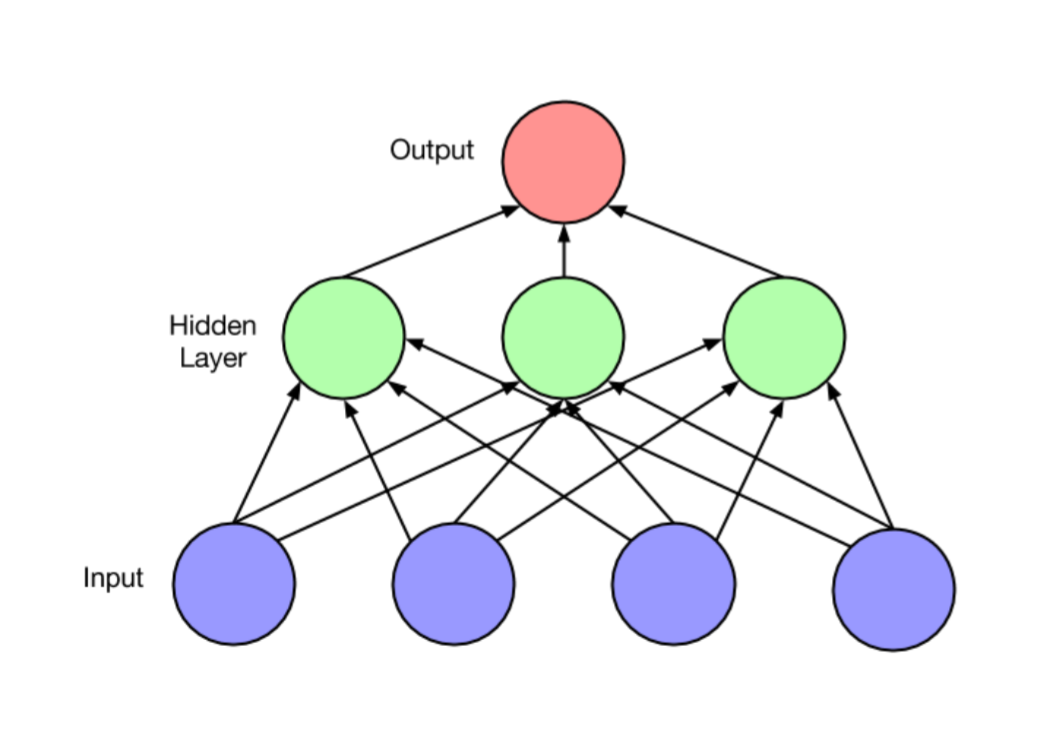
\includegraphics[width=0.6\linewidth]{basic_net.png}
\caption{A Basic Feed forward Neural Network.}
\label{fig:ANN}
\end{figure}

The most fundamental unit of a Neural Network is a neuron. A basic feed forward neural network consists of sets of neurons, commonly referred to as nodes, arranged into stacked layers \cite{ANN}. For a layer consisting of \(n\) individual nodes that is proceeded by a layer of \(m\) nodes, the number of connections that exist between the two layers is \(nm\). Each link between a node \(j'\) and a node \(j\), are assigned a set of trainable values, a weight \(w_{jj'}\) and a bias. Associated with each node is an activation function \(l_j(\cdot)\). The output value for node \(j\) is determined by passing the weighted sum of the inputs values through the activation function, such that:


\begin{equation}
v_j=l_j(\sum_{j'}w_{j'} \cdot v_{j'})
\end{equation}


This is represented on figure \ref{fig:node}, where the sigmoid activation function is denoted by \(\sigma\). 


\begin{figure}
\centering
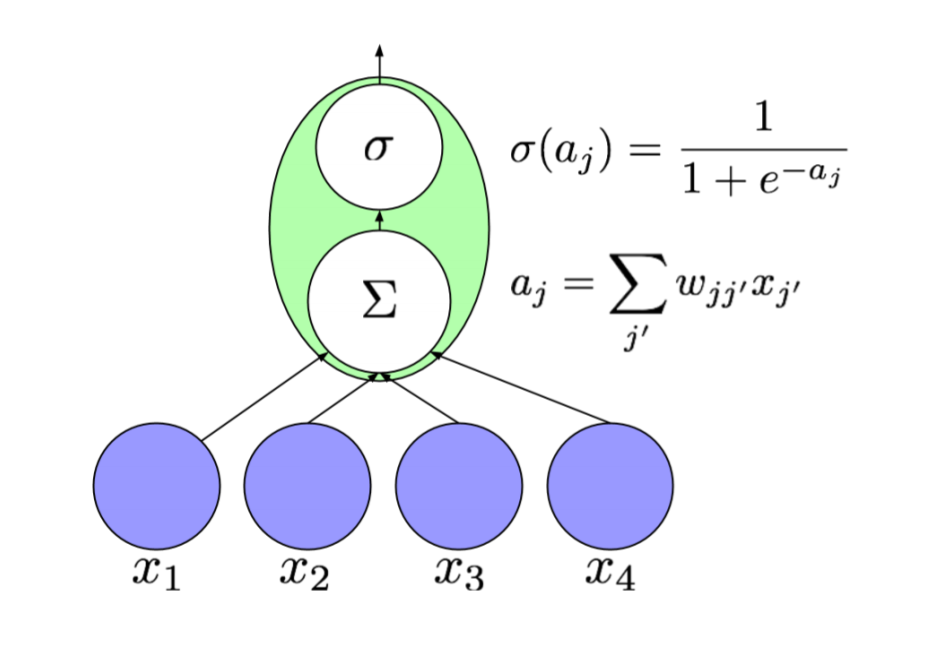
\includegraphics[width=0.7\linewidth]{node.png}
\caption{A node with a sigmoid activation function}
\label{fig:node}
\end{figure}


To train the network, input data that is labeled with a corresponding value or set of values that indicate the desired output is passed through the network. Initially, the network's weights and bias are random, thereby resulting in a random output. In order to train the network, we must find the optimal values for weights and biases that minimize the loss function, or error. This is accomplished through an optimization function. Back propagation is a highly successful gradient based optimization algorithm that operates by calculating the derivative of the loss function with respect to all the weights in the network \cite{LSTM2}.


The network learns by iterativily feeding training data through the network and updating the weights according to the loss function. Once the loss between the predicted value is close enough approximation to the correct output, when fed unseen data, the network can accurately approximate the correct output. 

\subsection{\label{sec:level2}Histogram of Orientated Gradients (HOG)}

HOG description

\section{Data and Software}

For the empirical application, we use 

(What do we use again?)

All data preparation, configuration, and management, is handled entirely within python 3.5, relying on the packages Numpy for array manipulation, Scipy for for HOG, and Skimage for it's implementations of legacy machine learning methods, such as Naïve Bayes, Random Forrest Trees, and Support Vector Machines. Neural Netowrks and Logistic Regressions were constructed using Keras, a high-level deep learning library for large scale machine learning, with Google's Tensorflow as a backend  

\section{Methodology} 

\section{Methodology} 

A core problem for quantitatively classify images is that in almost all cases there is no single feature that can be used to infer the class of the image. Human classification is a complicated and dynamic process build up through millions of years of evolution. First, we are easily able to identify if the object of interest is indeed within our field of vision. By observing an extremely minimal number of examples, we are able to intuitively infer features of importance to the object's class, subsequently allowing us to determine the class of an object by observing the degree to which each relevant feature is present, and taking a mentally weighted sum to determine which class it is most likely to belong to. It is extremely difficult to algorithmically mimic this approach.

Take the FR-I and FR-II classification task. Visually, the radio object's class is often clearly evident. Giving the FR-I galaxies frequently possess a few key features: the brightest points are always at the center of the source, the brightness usually changes more gradually, and brightness is usually inversely proportional to the distance from the sources.  FR-II radio galaxies, on the other hand, often comprise of two points that are equidistant from the source, form a strong linear correlation with the source, are often mirrored across the source, and are significantly brighter than the actual source itself. We could, in principle, take a single one of these features and build a classifier. Take the gradient for example. If the change in brightness for an FR-I source is, as a general rule, more gradual than that of an FR-II source, we can use this to determine a source's class. To illustrate: by taking the mean magnitude of the gradient for each pixel in a class for half the data, and then classifying the other half of the data based upon which value the mean gradient magnitude for each image is closest to gives an accuracy of 52.1\%. If we are to achieve an accuracy that is remotely within the range of human performance, we need to take into about all relevant features. While the degree to which these features are present in a sample can drastically vary, it is generally possible to classify a sample based upon a dynamic combination features. 

If we were to take this approach algorithmically, that is quantitatively determining the degree to which each of the relevant features exists and taking the weighted sum to determine the probability of the sample belong to either class, we would be feature engineering. This is not desirable. While theoretically capable of achieving high accuracies, many of the induvial features are extremely difficult to quantify, and are often areas of ongoing research in their own right. In addition, feature engineering is difficult to implement and is highly inflexible, making it hard to adapt to similar tasks. Due to these reasons, we instead take a machine learning based approach. 

Machine Learning techniques have been staggering successful in recent years for images classification. However, many of these algorithms, particularly state of the art methods such as convolutional neural networks, rely on vast amounts of images in order to extract useful features for classification. This makes them unsuited for tasks such as the FR-I/FR-II classification problem, where only 125 and 234 (or something) samples are known for the FR-I and FR-II classes respectively. We employ a number of methods to minimize this issue, primarily, by artificially increasing the number of samples. Using the ImageDataGenerator function in Keras, we applied a combination of random rotations, horizontal and vertical flips, horizontal and vertical translations, and zooms, allowing us to expand the dataset by a factor of one hundred. While genuine samples are preferable, this technique has been proven to be effective in the past (find sources).  Another method we employ is to convert the images into a format that allows less computationally exhaustive feature extraction. For this, we use HOG. 

\subsection{\label{sec:level2}Legacy Machine Learning Algorithms}
To establish a baseline for classification performance, we implement a Logistic Regression, Support Vector Machines (SVM), Naïve Bayes, and Random Forrest Trees (RFT).


\section{Results}

Results - lots of tables and graphs


\section{Discussion}




\section{Math and Equations}
Inline math may be typeset using the \verb+$+ delimiters. Bold math
symbols may be achieved using the \verb+bm+ package and the
\verb+\bm{#1}+ command it supplies. For instance, a bold $\alpha$ can
be typeset as \verb+$\bm{\alpha}$+ giving $\bm{\alpha}$. Fraktur and
Blackboard (or open face or double struck) characters should be
typeset using the \verb+\mathfrak{#1}+ and \verb+\mathbb{#1}+ commands
respectively. Both are supplied by the \texttt{amssymb} package. For
example, \verb+$\mathbb{R}$+ gives $\mathbb{R}$ and
\verb+$\mathfrak{G}$+ gives $\mathfrak{G}$

In \LaTeX\ there are many different ways to display equations, and a
few preferred ways are noted below. Displayed math will center by
default. Use the class option \verb+fleqn+ to flush equations left.

Below we have numbered single-line equations, the most common kind: 
\begin{eqnarray}
\chi_+(p)\alt{\bf [}2|{\bf p}|(|{\bf p}|+p_z){\bf ]}^{-1/2}
\left(
\begin{array}{c}
|{\bf p}|+p_z\\
px+ip_y
\end{array}\right)\;,
\\
\left\{%
 \openone234567890abc123\alpha\beta\gamma\delta1234556\alpha\beta
 \frac{1\sum^{a}_{b}}{A^2}%
\right\}%
\label{eq:one}.
\end{eqnarray}
Note the open one in Eq.~(\ref{eq:one}).

Not all numbered equations will fit within a narrow column this
way. The equation number will move down automatically if it cannot fit
on the same line with a one-line equation:
\begin{equation}
\left\{
 ab12345678abc123456abcdef\alpha\beta\gamma\delta1234556\alpha\beta
 \frac{1\sum^{a}_{b}}{A^2}%
\right\}.
\end{equation}

When the \verb+\label{#1}+ command is used [cf. input for
Eq.~(\ref{eq:one})], the equation can be referred to in text without
knowing the equation number that \TeX\ will assign to it. Just
use \verb+\ref{#1}+, where \verb+#1+ is the same name that used in
the \verb+\label{#1}+ command.

Unnumbered single-line equations can be typeset
using the \verb+\[+, \verb+\]+ format:
\[g^+g^+ \rightarrow g^+g^+g^+g^+ \dots ~,~~q^+q^+\rightarrow
q^+g^+g^+ \dots ~. \]

\subsection{Multiline equations}

Multiline equations are obtained by using the \verb+eqnarray+
environment.  Use the \verb+\nonumber+ command at the end of each line
to avoid assigning a number:
\begin{eqnarray}
{\cal M}=&&ig_Z^2(4E_1E_2)^{1/2}(l_i^2)^{-1}
\delta_{\sigma_1,-\sigma_2}
(g_{\sigma_2}^e)^2\chi_{-\sigma_2}(p_2)\nonumber\\
&&\times
[\epsilon_jl_i\epsilon_i]_{\sigma_1}\chi_{\sigma_1}(p_1),
\end{eqnarray}
\begin{eqnarray}
\sum \vert M^{\text{viol}}_g \vert ^2&=&g^{2n-4}_S(Q^2)~N^{n-2}
        (N^2-1)\nonumber \\
 & &\times \left( \sum_{i<j}\right)
  \sum_{\text{perm}}
 \frac{1}{S_{12}}
 \frac{1}{S_{12}}
 \sum_\tau c^f_\tau~.
\end{eqnarray}
\textbf{Note:} Do not use \verb+\label{#1}+ on a line of a multiline
equation if \verb+\nonumber+ is also used on that line. Incorrect
cross-referencing will result. Notice the use \verb+\text{#1}+ for
using a Roman font within a math environment.

To set a multiline equation without \emph{any} equation
numbers, use the \verb+\begin{eqnarray*}+,
\verb+\end{eqnarray*}+ format:
\begin{eqnarray*}
\sum \vert M^{\text{viol}}_g \vert ^2&=&g^{2n-4}_S(Q^2)~N^{n-2}
        (N^2-1)\\
 & &\times \left( \sum_{i<j}\right)
 \left(
  \sum_{\text{perm}}\frac{1}{S_{12}S_{23}S_{n1}}
 \right)
 \frac{1}{S_{12}}~.
\end{eqnarray*}
To obtain numbers not normally produced by the automatic numbering,
use the \verb+\tag{#1}+ command, where \verb+#1+ is the desired
equation number. For example, to get an equation number of
(\ref{eq:mynum}),
\begin{equation}
g^+g^+ \rightarrow g^+g^+g^+g^+ \dots ~,~~q^+q^+\rightarrow
q^+g^+g^+ \dots ~. \tag{2.6$'$}\label{eq:mynum}
\end{equation}

A few notes on \verb=\tag{#1}=. \verb+\tag{#1}+ requires
\texttt{amsmath}. The \verb+\tag{#1}+ must come before the
\verb+\label{#1}+, if any. The numbering set with \verb+\tag{#1}+ is
\textit{transparent} to the automatic numbering in REV\TeX{};
therefore, the number must be known ahead of time, and it must be
manually adjusted if other equations are added. \verb+\tag{#1}+ works
with both single-line and multiline equations. \verb+\tag{#1}+ should
only be used in exceptional case - do not use it to number all
equations in a paper.

Enclosing single-line and multiline equations in
\verb+\begin{subequations}+ and \verb+\end{subequations}+ will produce
a set of equations that are ``numbered'' with letters, as shown in
Eqs.~(\ref{subeq:1}) and (\ref{subeq:2}) below:
\begin{subequations}
\label{eq:whole}
\begin{equation}
\left\{
 abc123456abcdef\alpha\beta\gamma\delta1234556\alpha\beta
 \frac{1\sum^{a}_{b}}{A^2}
\right\},\label{subeq:1}
\end{equation}
\begin{eqnarray}
{\cal M}=&&ig_Z^2(4E_1E_2)^{1/2}(l_i^2)^{-1}
(g_{\sigma_2}^e)^2\chi_{-\sigma_2}(p_2)\nonumber\\
&&\times
[\epsilon_i]_{\sigma_1}\chi_{\sigma_1}(p_1).\label{subeq:2}
\end{eqnarray}
\end{subequations}
Putting a \verb+\label{#1}+ command right after the
\verb+\begin{subequations}+, allows one to
reference all the equations in a subequations environment. For
example, the equations in the preceding subequations environment were
Eqs.~(\ref{eq:whole}).

\subsubsection{Wide equations}
The equation that follows is set in a wide format, i.e., it spans
across the full page. The wide format is reserved for long equations
that cannot be easily broken into four lines or less:
\begin{widetext}
\begin{equation}
{\cal R}^{(\text{d})}=
 g_{\sigma_2}^e
 \left(
   \frac{[\Gamma^Z(3,21)]_{\sigma_1}}{Q_{12}^2-M_W^2}
  +\frac{[\Gamma^Z(13,2)]_{\sigma_1}}{Q_{13}^2-M_W^2}
 \right)
 + x_WQ_e
 \left(
   \frac{[\Gamma^\gamma(3,21)]_{\sigma_1}}{Q_{12}^2-M_W^2}
  +\frac{[\Gamma^\gamma(13,2)]_{\sigma_1}}{Q_{13}^2-M_W^2}
 \right)\;. \label{eq:wideeq}
\end{equation}
\end{widetext}
This is typed to show the output is in wide format.
(Since there is no input line between \verb+\equation+ and
this paragraph, there is no paragraph indent for this paragraph.)

\end{document}
%
% ****** End of file aipsamp.tex ******
